\chapter{Suunnittelu}
\label{ch:suunnittelu}
Tässä osuudessa käydään toteutetun ohjelman suunnittelu läpi ja kerrotaan miten ja miksi ratkaisuihin päädyttiin. Kappaleissa vertaillaan eri vaihtoehtoja ja peilataan kappaleessa \ref{ch:ongelmakohdat-ja-analysointi} käytyjä demoversion ongelmia ja niiden perusteella yritetään löytää toimiva ratkaisu. Ensin suunnitellusta ohjelmasta annetaan kattava kokonaiskuva lukijalle ja tämän jälkeen tulevissa kappaleissa mennään tarkemmin yksityiskohtiin.


\section{Kokonaiskuva}
Aikaisemmin kappaleessa \ref{ch:demoversio-ja-sen-toiminta} kuvassa \ref{fig:demo-architecture} esiteltiin demoversion arkkitehtuuri ja sen toiminta. Kuinka viestit IED-laitteelta kulkee ohjelman läpi ja tallennetaan tietokantaan. Kuinka järjestelmän muut komponentit lukevat tietoa tietokannasta kyselemällä sitä väliajoin ilman tietoa milloin uusi tieto on saapunut. Suunnittelun jälkeen demosta päädyttiin kuvassa \ref{fig:planned-system-architecture} olevaan arkkitehtuuriin. Kuvassa katkoviivalla on merkitty tässä kappaleessa suunniteltu ohjelmisto. Ja kuvan yläreunassa oleva viiva kuvaa viestin kulkua järjestelmän eri osapuolten läpi ja missä muodossa viesti on missäkin kohtaa. Kuvassa vasemmalla on IED-laite, josta komponentti viestit tilaa. Komponentti prosessoi ja julkaisee viestit RabbitMQ-välityspalvelimelle. Kuvassa oikealla järjestelmän muut komponenttit tilaavat viestejä välityspalvelimelta.

\begin{figure}[ht!]
	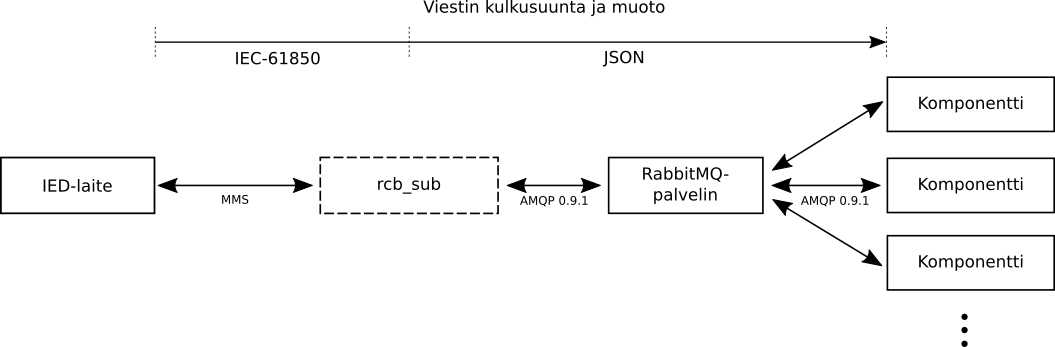
\includegraphics[width=1\textwidth]{pictures/planned-system-architecture.png}
	\caption{Suunnitellun komponentin toiminta ja viestin kulkeminen ja muoto osapuolten välillä.}
	\label{fig:planned-system-architecture}
\end{figure}

Komponentti päädyttiin toteuttamaan C-kielellä ja on komentorivipohjainen ohjelmisto. Komponentti ei käyttänyt tietokantaa vaan kaikki ohjelman ajoon annettavat parametrit annetaan komentoriviparametreille ennen ohjelman käynnistämistä. C-ohjelma voi tilata yhdellä IED-laitteella olevia RCB-instansseja. Tilattuaan RCB-instanssit, ohjelma odottaa viestejä IED-laitteelta IEC 61850 -standardin määrittämässä muodossa. Viestin saapuessa ohjelma prosessoi sen ja julkaisee AMPQ-standardin pohjaiselle välittäjäpalvelimelle \emph{JSON}-muodossa (engl. \emph{JavaScrip Object Notation}). Lopullisessa toteutuksessa välittäjäpalvelimena käytettiin RabbitMQ-nimistä ohjelmistoa, joka pohjautuu AMPQ-standrdin versioon 0.9.1. Välittäjäpalvelimelta muut järjestelmän komponentit voivat tilata viestejä, ja viestin saapuessa palvelin ilmoittaa siitä asiakkaalle. Toteutettu C-ohjelmisto käytti edelleen demoversiosta tuttua libiec61850-kirjastoa hoitamaan matalan tason IEC 61850 -standardin määrittämän funktionaalisuuden.


\section{Järjestelmän hajautus ja arkkitehtuuri}
\label{ch:järjestelmän-hajautus-ja-arkkitehtuuri}

Komponentille vaatimuksena oli järjestelmän hajauttamisen mahdollistaminen. Komponentti pitäisi olla oma kokonaisuutensa ja sen ei tarvitse tietää mitään muista järjestelmän komponenteista.  Järjestelmän hajautus tarkoittaa järjestelmän osittamista pieniin omiin kokonaisuuksiinsa, jotka kommunikoivat keskenään esimerkiksi viestien välityksellä. Demossa erilliset ohjelmat joutuivat jatkuvasti lukemaan viestejä tietokannasta, ilman tietoa siitä milloin uusi viesti oli saatavilla. Tällainen ratkaisu ei ollut hyvä järjestelmän hajautuksen näkökulmasta. Tilanne pahenisi jos tietoa tarvitsevia järjestelmän komponentteja olisi enemmän. Lisäksi tässä toteutuksessa tietokanta on jatkuvan lukemisen alaisena. Tilanteeseen tarvittiin ratkaisu, jossa järjestelmän osa voisi tilata tietoa ja saada ilmoituksen kun tieto on saatavilla. Toisin sanoen tilaaja-julkaisija -arkkitehtuurimalli.

Yhtenä ratkaisuna tilanteeseen jossa moni komponentti tarvitsee samaa tietoa, olisivat ne voineet suoraan tilata viestit IED-laitteelta. Näin kaikki tilaajat saisivat saman viestin. Kuitenkin tässä esteenä on, että IEC 61850 -standardin määrityksen mukaan yksi RCB-instanssi voi olla vain tilattuna yhdellä asiakkaalle kerrallaan, niin kuin teorian kappaleessa \ref{ch:viestien-tilaus-ja-tilauksen-konfigurointi} käsiteltiin. Ja IED-laitteiden RCB-instanssit ovat rajalliset ja päätetty laitteen konfiguroinnin yhteydessä. Lisäksi IED-laitteet pystyvät rajoittamaan päällä olevien yhteyksien määrää johonkin lukuun, joka voi olla pieni. Tavoitteena siis olisi minimoida avoimet yhteydet IED-laitteelle, ja samalla tarjota saapunut viesti mahdollisimman monelle siitä kiinnostuneelle osapuolelle. Näistä vaatimuksista päästään ratkaisuun, missä yksi ohjelma tilaa kaikki halutut RCB-instanssit yhdeltä IED-laitteelta. Odottaa viestien saapumista ja lähettää ne edelleen muille niitä tarvitseville ohjelmille. Viestejä tarvitsevien ohjelmien määrä voi vaihdella tarpeen mukaan. Tästä päästään vaatimukseen, että IED-laitteelta viestejä tilaavan ohjelmiston ei tarvitsisi tietää muista tilaavista ohjelmista mitään. Ohjelman pitäisi pystyisi julkaisemaan viestit eteenpäin, välittämättä siitä kuka viestejä vastaanottaa.

Ratkaisuna yllä mainittuihin vaatimuksiin oli sijoittaa IED-laitteen ja muiden järjestelmän osien väliin \emph{väliohjelmisto} (engl. \emph{middleware}), kuten kuvassa \ref{fig:planned-system-architecture} C-ohjelma on sijoitettu. Tällä pystyttiin minimoimaan yhteyksien määrä IED-laitteelle yhteen. Lisäksi sijoittamalla C-ohjelman ja muiden järjestelmän komponenttien väliin välittäjäpalvelin, saatiin aikaan joustavuus mitä vaatimuksissa asetettiin. C-ohjelman ei tarvitse välittää siitä kuka viestejä vastaanottaa ja välittäjäpalvelimen avulla yhden julkaisijan viestit voi tilata monta erillistä tilaaja. Välittäjäpalvelimelta jokainen tilaaja saa saman alkuperäisen viestin, mutta kopiona. IEC 61850 -standardi määritti vain tilaaja-julkaisija arkkitehtuurimallin ainoaksi tavaksi saada viestejä. Niinpä väliohjelmiston toteuttaminen ja saman arkkitehtuurin jatkaminen järjestelmän muille osille on tilanteeseen sopiva arkkitehtuurimalli. Tämä suunnitelma arkkitehtuurista täytti kaikki sille asetetut vaatimukset ja todettiin toimivaksi. Lisäksi nämä päätökset vastaavat kappaleessa \ref{ch:johdanto} asetettuun tutkimuskysymykseen, mikä arkkitehtuurimalli sopisi parhaiten tähän tilanteeseen sopivaksi. Myös kysymykseen kuinka järjestelmä hajautetaan niin että tiedon siirto eri osapuolten välillä olisi mahdollista ja joustavaa saatiin vastaus. Vastaus tähän kysymykseen on käyttää jotakin viestintäprotokollaa, jonka kaikki osapuolet voivat ymmärtää. Arkkitehtuurissa käytettiin AMQP-viestintäprotokollaa, joka mahdollista yhteiset säännöt ja kommunikoinnin eri osapuolten välillä. Viestintä on yleinen tapa kommunikoida hajautetussa järjestelmässä \mbox{\cite[s.~2]{distributed-systems-concepts-and-design}}. Ratkaisu todettiin hyväksi ja toimivaksi.

Demoversiossa ohjelma luki IED-laitteen tiedot kuten IP-osoitteen ja RCB-instanssien viitteet tietokannasta ja tallensi saapuneet viestit myös tietokantaan. Uudessa arkkitehtuurissa viestit julkaistiin erilliselle välittäjäpalvelimelle, jonka ansiosta tietokantaa ei enää tähän tarvittu. C-ohjelman tarkoitus oli olla väliohjelma viestien välittämiseen eteenpäin, joten siihen ei tarvittu käyttöliitymää. Ohjelmasta päätettiin toteuttaa komentorivipohjainen, jolle kaikki tiedot voitaisiin syöttää komentoriviparametereillä käynnistyksen yhteydessä. Näillä muutoksilla tietokanta voitiin jättää kokonaan pois riippuvuuksista.


\section{Suorituskyky ja kielen valinta}
Demoversio oli ohjelmoitu Ruby-kielellä ja siinä oli paikoin suoritukseen liittyviä ongelmia ja epävarmuutta, etenkin viestien ja RCB-instassien määrän ollessa suurempi. Demon toimintaa ja ongelmia käytiin läpi aikaisemmin kappaleessa \ref{ch:ongelmakohdat-ja-analysointi}. Suorituskyvyn ja toiminnan epävarmuuden takia demo ei ollut tuotantovalmis, vaan vaati parannuksia. Ennen kuin päädyttiin kirjoittamaan koko ohjelma uudestaan eri tekniikalla, kokeiltiin demoa korjata vaihtamalla Ruby-tulkkia. Rubyn MRI-oletustulkki yritettiin vaihtaa \emph{JRuby}-tulkkiin \cite{jruby-homepage}. Tavoitteena vaihdossa oli saada Ruby-ohjelma toimimaan ilman globaalia tulkkilukitusta, eli GIL:ilä. GIL:iä käsiteltiin aikaisemmin kappaleessa \ref{ch:ongelmakohdat-ja-analysointi}. JRuby on Ruby-tulkki, joka suorittaa Ruby-koodia \emph{Java-virtuaalikoneen} (engl. \emph{Java Virtual Machine}, lyhennetään \emph{JVM}) avulla. JRuby mahdollistaa säikeiden suorituksen rinnakkain JVM:n omilla säikeillä ja näin ollen suorituksen pitäisi olla nopeampaa \mbox{\cite{Youssef2013}}. Aidolla rinnakkaisuudella ohjelman suoritus ei olisi pysähtynyt viestin saapuessa takaisinkutsufunktion suorituksen ajaksi. LibEIC61850-kirjasto kutsuu asetettua takaisinkutsufunktioa viestin saapuessa, joka prosessoi viestin ja tallentaa sen tietokantaan. Tämä ei olisi kuitenkaan ratkaissut kaikkia ohjelmassa olevia ongelmia, kuten muistivuotoa ja hitaampaa suoritusta verrattuna käännettävään kieleen. Tämä toteutus ei kuitenkaan toiminut ja nopean yrityksen jälkeen päätettiin vain palata suunnitelmaan kirjoittaa koko ohjelma uudestaan. Lisäksi demon arkkitehtuuri olisi silti pitänyt viedä saman suuntaan kuin kappaleessa \ref{ch:järjestelmän-hajautus-ja-arkkitehtuuri} kuvattiin. Demo oli toteutettu osaksi isompaa RoR-projektia, joka toimi Rubyn-oletustulkin päällä. JRuby ei tukenut kaikkia projektin käyttämiä kirjastoja. Tämä oli pääsyynä miksi JRuby:n ei päädytty. Rubyssä kirjastoja kutsutaan \emph{jalokiviksi} (engl. \emph{gem}). Seurauksena olisi ollut saman projektin ylläpitäminen kahdelle eri tulkille tai asennettavien kirjastojen erottaminen. Lopulta tähän vaihtoehtoon ei päädytty ja lisäksi täytyi ottaa huomioon implementaatioon käytetty aika ja useat mahdolliset viat jotka olisi silti pitänyt demosta korjata. Kaikkiaan oli vain helpompaa kirjoittaa ohjelma alusta kokonaan uudella tekniikalla. Samalla uudelle toteutuksessa asetetut tavoitteet tiedettiin ja kuinka demossa olevat ongelmat pystyttiin välttämään. Demon uudelleenkirjoittamiseen ja korjaamiseen käytetty aika voitiin käyttää kokonaan uuden toteutuksen kirjoittamiseen.

Uuden toteutuksen kieleksi valittiin C-kieli. Isona syynä kielen valintaan oli tekijän iso mieltymys matalan tason ohjelmointiin ja C-kieleen. Lisäksi C-kieli käännetään alustalle suoraan konekäskyiksi, joiden suoritus on nopeampaa kuin tulkattavan kielen, kuten Ruby ja Python. Kielen valinnan yhteydessä kuitenkin oli hyvä varmistaa kaikkien suunniteltujen liitosten mahdollisuus. C-kielelle löytyi kirjastoja RabbitMQ-välittäjäpalvelimen käyttämiseen ja lisäksi JSON-rakenteen muodostamiseen. Hyötynä vielä C-kielen valinnasta oli, että demossa käytettyä libIEC61850-kirjastoa pystyttiin käyttämään suoraan ilman erillistä liitosta, koska kirjasto oli myös tehty C-kielellä. Tarkemmin käytettyihin kirjastoihin ja toteutukseen mennään kappaleessa \ref{ch:toteutus}.

Tutkimuskysymykseen jossa etsittiin vastausta siihen, mikä aiheutti demon ongelmia ja kuinka niitä voisi estää saatiin vastaus. Vastauksia syihin saatiin aikaisemmin kappaleessa \ref{ch:ongelmakohdat-ja-analysointi}. Valitsemalla eri tekniikat kuten C-kieli, vastataan osittain kysymykseen kuinka suorityskykyongelma ja toiminnan epävarmuus vältetään. Muistivuotoa vältetään huolellisella ohjelmoinnilla ja testaamisella. Tiedon jakamisen ongelma liittyy osin järjestelmän hajauttamisen kysymykseen. Molempiin kysymyksiin vastaus on ottaa käyttään erillinen välittäjäpalvelin viestien välitykseen järjestelmässä eri osapuolten kesken.


\section{Prosessoidun viestin muoto ja rakenne}
Saapuva viesti esitetään libIEC61850-kirjastossa \emph{ClientReport}-struktuurin instanssina. Stuktuuri sisältää viestin datan ja sen voi lukea käyttämällä kirjaston tarjoamia funktioita \mbox{\cite{libIEC61850-doc}}. Saapunut viesti haluttiin jakaa välittäjäpalvelimen läpi muille osapuolille, joten viestin täytyi olla helposti luettavassa muodossa muille ohjelmille. Viesti päädyttiin muuttamaan helposti ymmärrettäväksi JSON-rakenteeksi. JSON-rakenteen voi helposti ihminen lukea ja se on nykypäivänä paljon käytetty tiedonsiirtomuoto erilaisissa web-palveluissa ja rajapinnoissa. Myöskin JSON-rakenteiden lukemiseen on monelle eri kielellä olemassa valmiita kirjastoja sen monikäyttöisyyden takia \mbox{\cite{Patrizio2016}}.

Liitteessä \ref{ch:report-json-format} on esitetty C-ohjelman viestistä muodostettu JSON-rakente. Saman JSON:in C-ohjelmaa julkaisi RabbitMQ-välittäjäpalvelimelle. Standardin määrittämää viestin rakennetta ja sisältöä käytiin läpi kappaleessa \ref{ch:viestin-rakenne}. JSON:in rakenne noudattaa pääosin standardin määrittämää viestin rakennetta. C-ohjelma lisäsi viestiin attribuuteihin sen viitteen, tyypin ja koon. Nämä tiedot eivät ole standardin määrittämässä viestissä ja ne todettiin tarpeelliseksi tiedoksi muille järjestelmän osille jotka viestejä lukevat. Tiedot luetaan ja selvitetään IED-laitteelta erillisillä palvelukutsuilla ennen tilauksen aloittamista. Nämä tiedot yhdistetään viestin saapuessa JSON-rakenteeseen. Tätä käsitellään tarkemmin kappaleessa \ref{ch:toteutus}.

Standardin viestin kenttien määrää pystyi säätämään RCB-instanssin \emph{OptFlds}-attribuutilla. JSON:iin kuitenkin haluttiin lisätä kaikki mahdolliset kentät selkeyden vuoksi. Jos kenttä puuttui viestistä, asetettiin sen arvoksi JSON:issa \emph{null}-arvo. Esimerkiksi liitteessä \ref{ch:report-json-format} kentän confRevision arvo on null. Tällöin RCB-instanssissa OptFlds-attribuutin \emph{conf-revision}-bitti on ollut epätosi. Sama toistettiin kaikille muillekin vaihtoehtoisille kentille. Tällä periaatteella viestin OptFlds-kenttä voitiin jättää pois JSON:ista. JSON:iin päädyttin lisäämään FCD- ja FCDA-viitteiden alla viitatut oikeat attribuutien viitteet, tyyppit ja koot. Tämä toteutettiin selkeyden takia ja näin voidaan päätellä mitkä arvot oikeasti kuuluvat viestiin ja mitkä ovat niiden viitteet. Standardissa viesti sisälsi vain datajoukon FCD- tai FCDA-viitteen ja taulukon arvoja mihin attribuutteihin sen alla viitattiin. JSON:iin tämä taulukon arvot on avattu ja jokaiselle taulukon arvolle on lisätty sen viite, tyyppi ja koko. Liitteessä \ref{ch:report-json-format} oleva JSON-rakenne koostuu kahdesta sisäkkäisestä values-taulukosta (rivit 7 ja 13). Rivillä 7 oleva values-taulukko sisältää viestissä olevat datajoukon FCD- tai FCDA-viitteet ja niihin liittyvät kentät. Samalla periaattelle kuin standardin määrittämässä viestin rakenteessa kuvassa \ref{fig:iec61850-report-format} olevat taulukon arvot 1--n:ään. Eli viestin \emph{Reason Code} on laitettu \emph{reasonForInclusion} attribuuttiin. Viestin \emph{DataRef}-kenttä on pilkottu kolmeen eri kenttään \emph{mmsReference}, \emph{reference} ja \emph{functionalConstraint}. Viestien viitteet tulevat MMS-protokollamäärityksen muodossa, eli pisteet (.) on korvattu dollari-merkillä (\$) ja viite sisältää funktionaalisen rajoitteen. Nyt mmsReference sisältää viestin alkuperäisen MMS-viitteen, reference sisältää standardin abstraktin viitteen ja functionalConstraint sisältää funktionaalisen rajoitteen. Nämä on erotettu selkeyden takia, koska mahdollisesti jotkin komponentit saattavat tarvita standardin käyttämää abstraktia viitettä ja näin välttää teksimuunnokset. JSON:in sisempi values-attribuutti (liitteessä \ref{ch:report-json-format} ensimmäinen rivillä 13) sisältää viestistä avatun arvo-taulukon. Jokaisen taulukon arvoon on lisätty sen koko viite, tyyppi ja koko. Poikkeuksena \emph{boolean} ja \emph{utc-time} tyypit, jolla ei ole kokoa ollenkaan. Koko kertoo monellako bitillä kyseinen attribuutti esitetään ja se voi vaihdella saman tyypin välillä, esimerkiksi \emph{bit-string}. Myöskin bit-string-tyypille päädyttiin lisäämään kaksi eri arvoa \emph{valueLittleEndian} ja \emph{valueBigEndian}. Attribuutista riippuen, sen tavujärjestys voi olla eri. Tämän takia päätettiin tarjota tilaajalle molemmat vaihtoehdot. Ajat päätettiin antaa suoraan samassa formaatissa kuin viestissä. Viestin päätason aikaleima on millisekunteja \emph{UNIX}-ajanlaskun alusta 1. tammikuuta 1970 klo 00:00:00 UTC tähän hetkeen. Attribuuteissa tyypiltään utc-time, luku on sekunteja samasta UNIX-ajanlaskusta tähän hetkeen \mbox{\cite[s.~26--27]{IEC61850-7-2}}.

Tutkimuskysymykseen jossa etsittiin vastausta kysymykseen mikä olisi sopiva tiedon jakamisen muoto hajautetussa järjestelmässä. Vastauksena kysymykseen tässä työssä valittiin JSON. JSON on nykypäivänä web-ohjelmoinnissa paljon käytetty tiedon jakamisen muoto rajapinnoissa. Toinen vaihtoehto olisi ollut XML-muoto, mutta se on raskaampi kuin JSON ja ei niin helposti ihmisen luettavissa. JSON-muodon on ihmiselle helposti luettavissa ja ymmärrettävissä. Lisäksi JSON:in lukuun monelle eri kielelle on olemassa valmiita kirjastoja sen yleisyyden takia. JSON:in valinta todettiin hyväksi ja toimivaksi ratkaisuksi. \cite{the-rise-and-rise-of-json, why-json-is-better-than-xml}